%% LaTeX Beamer presentation template (requires beamer package)
%% see http://bitbucket.org/rivanvx/beamer/wiki/Home
%% idea contributed by H. Turgut Uyar
%% template based on a template by Till Tantau
%% this template is still evolving - it might differ in future releases!

\documentclass{beamer}

\usepackage{calc,verbatim}
\usepackage{movie15}
%\usepackage{multimedia}

\usepackage{tikz}
\usetikzlibrary{fit}
\usetikzlibrary{backgrounds}
\usetikzlibrary{trees,positioning}
\usetikzlibrary{shapes.geometric,shapes.symbols}

\usepackage{pgfplots}
\pgfplotsset{compat=newest}

% Setup appearance:

\usetheme{Frankfurt}

\usefonttheme[onlylarge]{structurebold}
%\usefonttheme{structurebold}
\setbeamerfont*{frametitle}{size=\normalsize,series=\bfseries}
\setbeamertemplate{navigation symbols}{}

\definecolor{ubcblue}{RGB}{0,40,89}
\definecolor{ubcgray}{RGB}{116,145,163}

\setbeamercolor{section in toc}{fg=ubcblue,bg=white}
\setbeamercolor{alerted text}{fg=ubcblue}
\setbeamercolor*{palette primary}{fg=white,bg=ubcblue}
\setbeamercolor*{palette secondary}{fg=ubcblue,bg=ubcblue}
\setbeamercolor*{palette tertiary}{fg=white,bg=ubcblue}
\setbeamercolor*{palette quaternary}{fg=ubcgray!50!white,bg=ubcblue}

%\setbeamercolor*{sidebar}{fg=ubcblue,bg=gray!15!white}

%\setbeamercolor*{palette sidebar primary}{fg=ubcblue!10!black}
%\setbeamercolor*{palette sidebar secondary}{fg=white}
%\setbeamercolor*{palette sidebar tertiary}{fg=ubcblue!50!black}
%\setbeamercolor*{palette sidebar quaternary}{fg=ubcgray!10!white}

%\setbeamercolor*{titlelike}{parent=palette primary}
%\setbeamercolor{titlelike}{parent=palette primary}
%\setbeamercolor{frametitle}{fg=white,bg=ubcgray}
%\setbeamercolor{frametitle right}{bg=ubcgray!60!white}

%\setbeamercolor*{separation line}{green}
%\setbeamercolor*{fine separation line}{red}


\setbeamercolor{item projected}{bg=ubcblue}
\setbeamercolor{block title}{bg=ubcgray}
\setbeamercolor{block body}{bg=ubcgray!20!white}
\setbeamercolor{description item}{fg=ubcblue}
\setbeamercolor{caption name}{fg=ubcblue}

\setbeamerfont*{frametitle}{size=\Large}
\setbeamerfont*{title}{size=\Large}
\setbeamerfont*{section in toc}{size=\large}
\setbeamerfont*{block title}{}

\usepackage[english]{babel}
\usepackage[latin1]{inputenc}

% font definitions, try \usepackage{ae} instead of the following
% three lines if you don't like this look
%\usepackage{mathptmx}
%\usepackage[scaled=.90]{helvet}
%\usepackage{courier}
\usepackage{times}


\usepackage[T1]{fontenc}

% Setup TikZ

\usepackage{tikz,pgfplots,siunitx}
\usetikzlibrary{arrows,fadings,spy,fit,positioning}
%\pgfplotsset{every extra y tick/.append style={grid style=black}}
\usetikzlibrary{positioning,decorations,fit,backgrounds,scopes,calc,decorations.pathreplacing}
\usetikzlibrary{shapes.geometric}

\setbeamertemplate{footline}{
\normalfont 
\leavevmode
\hbox{
\begin{beamercolorbox}[wd=.98\paperwidth,ht=2.5ex,dp=2.125ex,leftskip=.3cm,rightskip=.3cm]{title in head/foot_}
\insertauthor
\hfill 
\insertshorttitle
\hfill
\insertframenumber
   \end{beamercolorbox}
}
}

%\newcommand{\watermarklogo}{
\includegraphics[width=5.5cm,trim=1.5cm 1.5cm 1.5cm
%1.5cm]{images/ovgu_logo.pdf}}
\newcommand{\watermarklogo}{
\includegraphics[width=4.8cm]{images/ubcblue.png}}

\usebackgroundtemplate{
\parbox[b][\paperheight+1.75cm]{\paperwidth+1cm}{
	\hfill\tikz 
	\node {\watermarklogo}
	node[fill=white,path fading=south,fading angle=45] {\phantom{\watermarklogo}}%
	node[fill=white,opacity=0.26] {\phantom{\watermarklogo}};
}
}

%\endofdump

\title{DarkVR: The Virtual Blind Reality}

%\subtitle{}

% - Use the \inst{?} command only if the authors have different
%   affiliation.
%\author{F.~Author\inst{1} \and S.~Another\inst{2}}
\author{Tom Brosch}

% - Use the \inst command only if there are several affiliations.
% - Keep it simple, no one is interested in your street address.
\institute[Universities of British Columbia]
{
Electrical and Computer Engineering\\
University of British Columbia
}

\date{Human Interface Technologies 2012 Conference}


% This is only inserted into the PDF information catalog. Can be left
% out.
\subject{Talks}



% If you have a file called "university-logo-filename.xxx", where xxx
% is a graphic format that can be processed by latex or pdflatex,
% resp., then you can add a logo as follows:

% \pgfdeclareimage[height=0.5cm]{university-logo}{university-logo-filename}
% \logo{\pgfuseimage{university-logo}}



% Delete this, if you do not want the table of contents to pop up at
% the beginning of each subsection:
%\AtBeginSubsection[]
%{
%\begin{frame}<beamer>
%\frametitle{Outline}
%\tableofcontents[currentsection,currentsubsection]
%\end{frame}
%}

% If you wish to uncover everything in a step-wise fashion, uncomment
% the following command:

%\beamerdefaultoverlayspecification{<+->}

\begin{document}

\begin{frame}
\titlepage
\end{frame}

\begin{frame}{Outline}
\tableofcontents
% You might wish to add the option [pausesections]
\end{frame}


\section{Introduction}

\subsection{Motivation}

\begin{frame}{Motivation}

Inspired by \textsc{Dialogue in the
Dark}\footnote{\url{http://www.dialogue-in-the-dark.com/}}
\begin{columns}
\column{0.6\textwidth}
\begin{itemize}
  \item Indoor Exhibition
  \item 100\% darkness
  \item Guided by visually impaired
  \item Learn to trust your other 4 senses 
\end{itemize}
\column{0.31\textwidth}

\includegraphics[width=\columnwidth]{images/dialog2}
\end{columns}
\vspace{0.5em}
\begin{block}{Goal}
\begin{itemize}
  \item Create a unique experience
  \item Raise awareness for the problems of visually impaired
\end{itemize}
\end{block}

\end{frame}

\subsection{Overview}

\begin{frame}{Video Demo}

\begin{center}
%\includemovie[poster,text={
%
\includegraphics[width=8cm,
% height=6cm]{images/bbb-splash-thumb.png}},mouse=true]{8cm}{6cm}{videos/bbb.wmv}
%\movie{
\includegraphics[width=8cm,
% height=6cm]{images/bbb-splash-thumb.png}}{videos/eece518.wmv}
\includemovie[poster]{8cm}{6cm}{videos/eece518.wmv}
\end{center}

\end{frame}

\begin{frame}{Component Summary}

\begin{center}
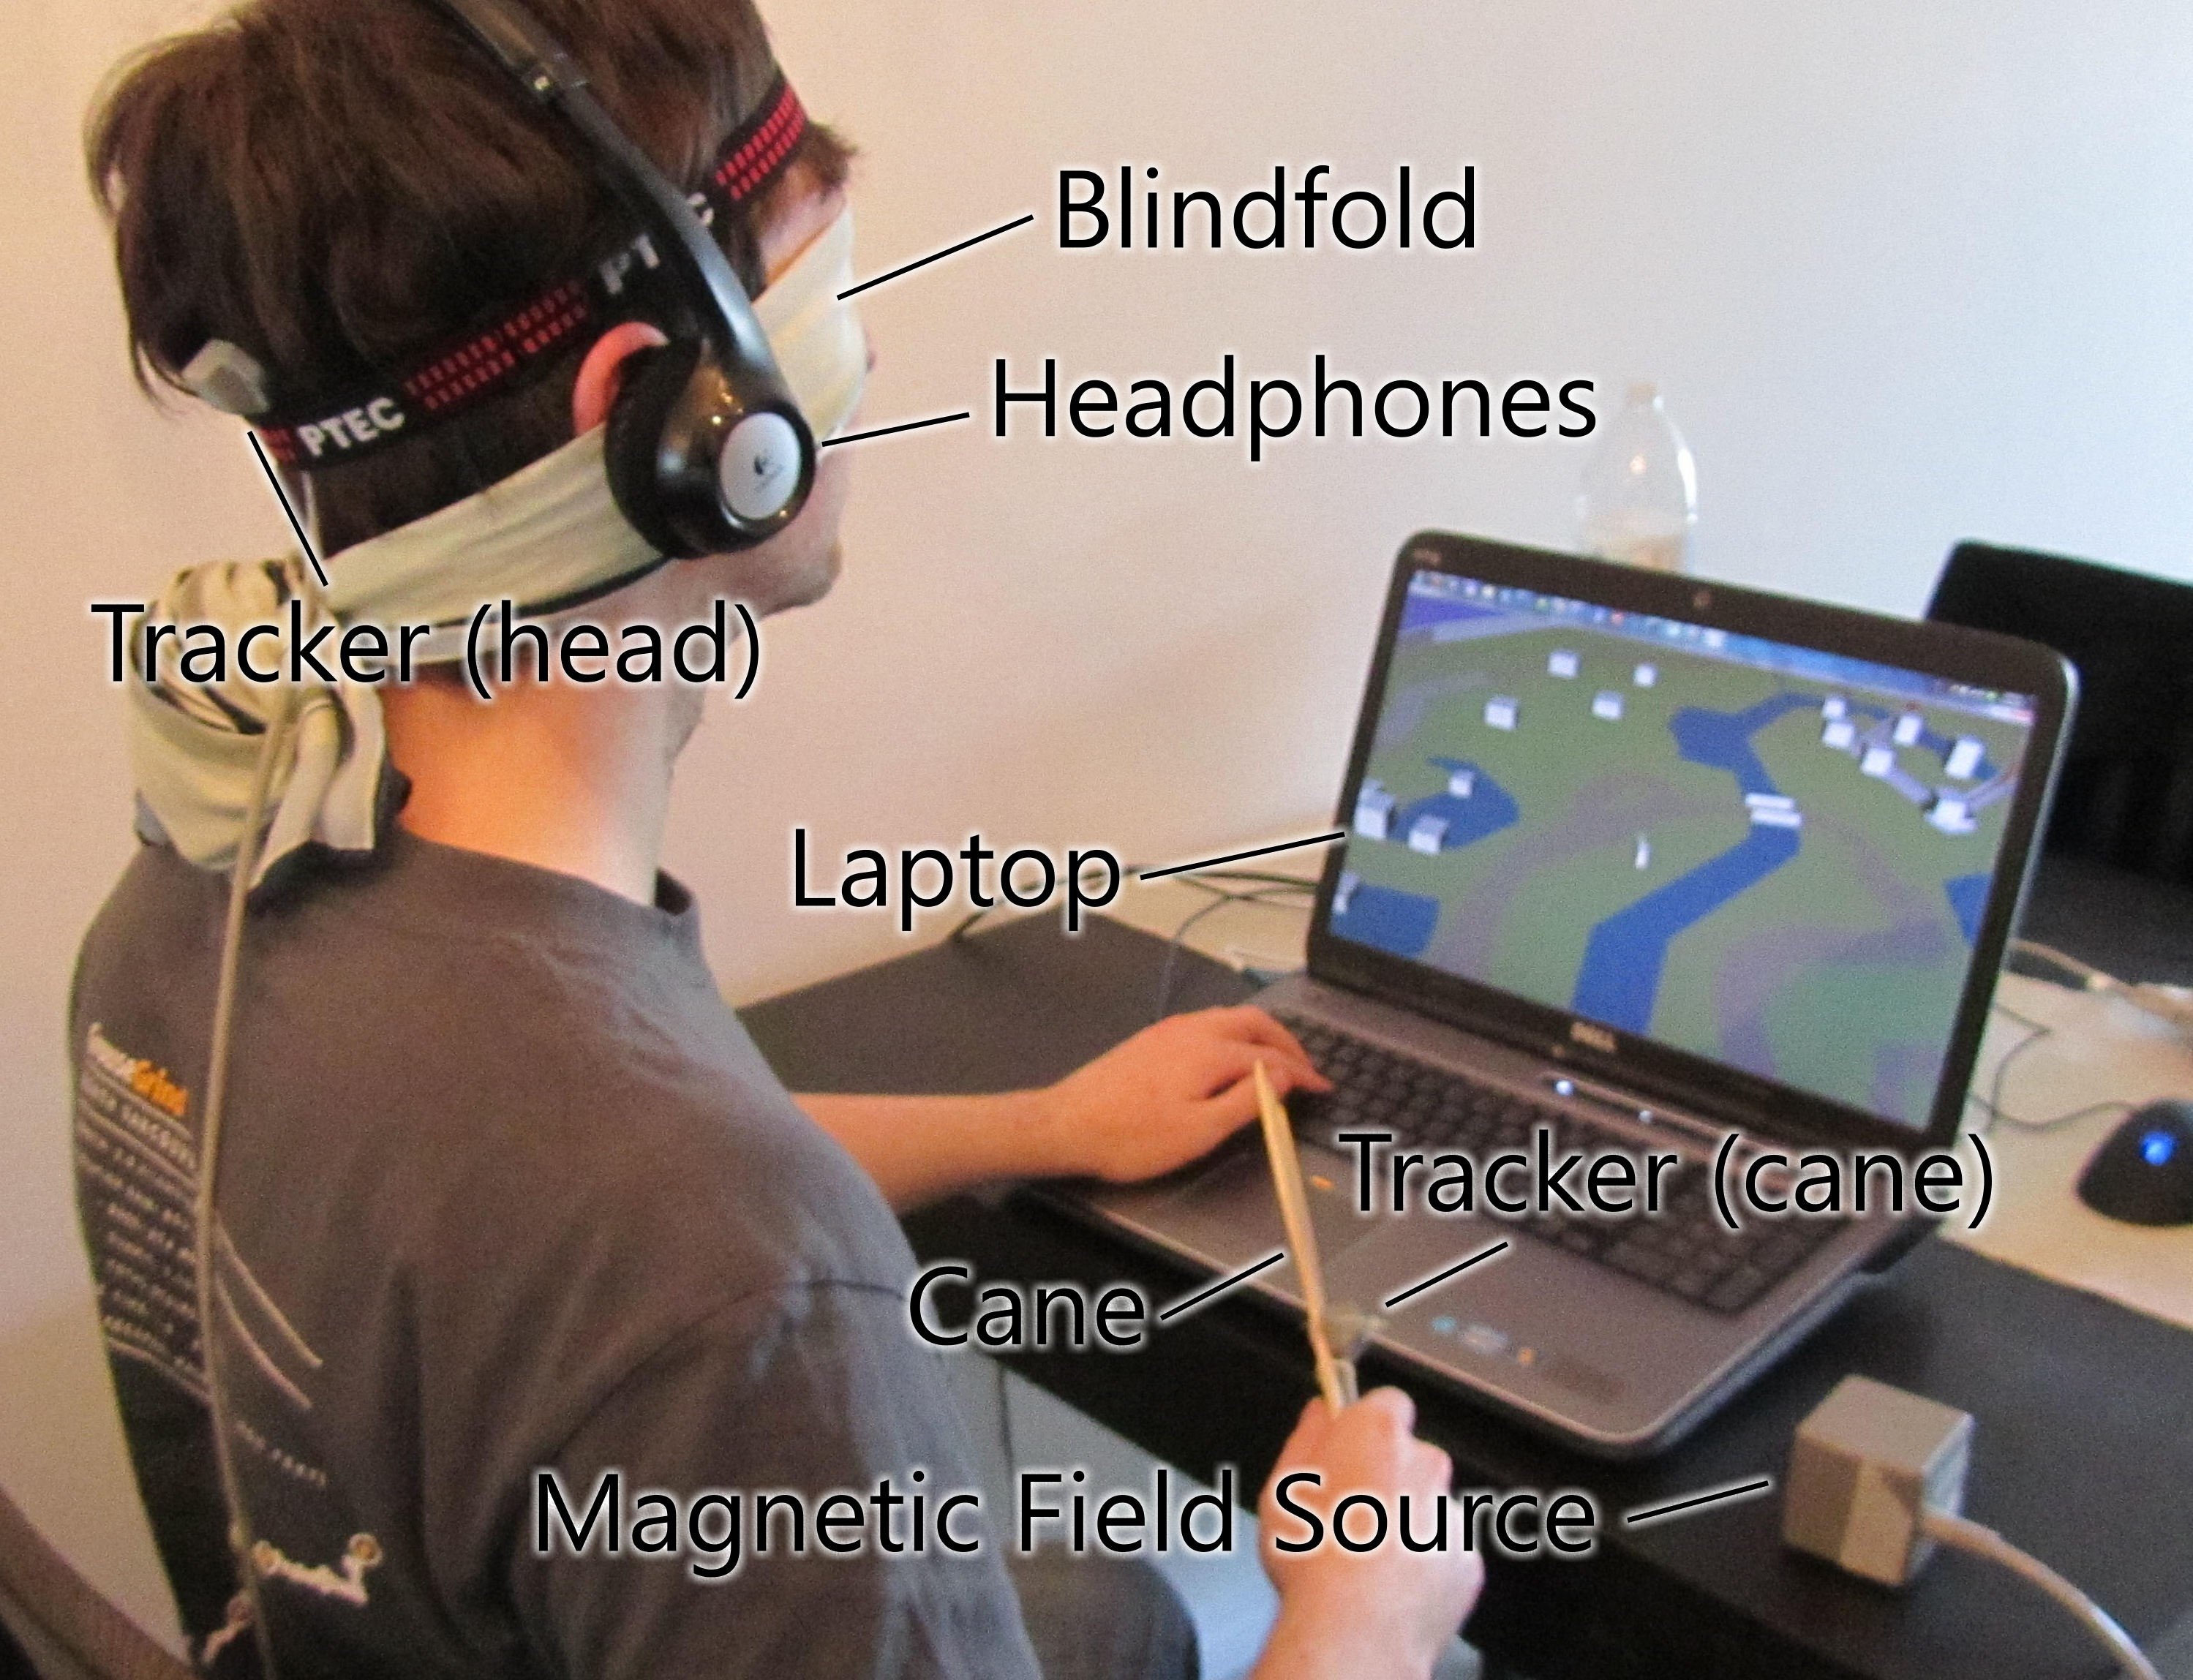
\includegraphics[width=0.7\textwidth]{images/details2}
\end{center}

\end{frame}

\section{Method}

\subsection{The DarkVR System}

\begin{frame}{System Overview}

\begin{block}{Hardware Components}
\begin{itemize}
  \item Tracker system
  \item Laptop
  \item Cane
\end{itemize}
\end{block}

\begin{block}{Software Components}
\begin{itemize}
  \item World Model (SceneGraph)
  \item Sound Engine
  \item Collision Engine
  \item Input Controllers
\end{itemize}
\end{block}

\end{frame}

\begin{frame}[fragile]{System Architecture}

\tikzstyle{every node}+=[font=\sffamily]

\begin{center}
\begin{tikzpicture}[transform canvas={xshift=1.7cm,yshift=-1cm,scale=0.8}]

\tikzstyle{data}=[minimum height=2.8cm,
	minimum width=1.5cm,
	cylinder,draw, rotate=90, shape
	aspect=0.4, align=center]
	
\tikzstyle{input}=[draw,signal,signal from=west, signal to=east,
align=center,fill=white]

\tikzstyle{procedure}=[draw,trapezium,trapezium left angle=45, trapezium
right angle=-45,align=center]

\matrix[column sep={2cm,between origins}] (datamatrix)
{ 
\node<1-> {}; & \node<1-> {}; & \node<1>[font=\color{white}]{Data};
\node<2->{Data}; & \node<1-> {}; & \node<1-> {};
\\[1em] 
\node<2->[data] (avatar) {Avatar\\ Model};
	& \node<1->[data] {Scene\\ Graph};
	& \node<1->[data] {Collision\\ World};
	& \node<1->[data] {FMOD 3D\\ Geometry}; 
	& \node<2->[data] {Program\\ Parameters}; \\
};

\node<2->[fit=(datamatrix), draw, inner sep=10pt, rounded corners,
dashed] (databox) {};

\node<3->[input, left=1.8cm of avatar.north] (keyboard){Keyboard\\
Input};
\node<3->[procedure, above=of databox,draw=white,font=\color{white}]
(callbacks2) {Update Callbacks\\
(Body, Head, Cane)};
\node<3->[input] (tracker) at (keyboard|-callbacks2) {Trackers};
\draw<3->[->] (keyboard)--node[above=2pt,fill=white,inner
sep=1pt]{changes}(avatar);

\node<4->[procedure, above=of databox] (callbacks) {Update Callbacks\\
(Body, Head, Cane)};
\draw<4->[<-] (tracker)--node[above]{read from} (callbacks);
\draw<4->[<->] (callbacks)--node[right]{update (read + write)}(databox);

\end{tikzpicture}
\end{center}

\end{frame}

\subsection{World Design}

\begin{frame}{The Environments}

\begin{columns}
\column{0.5\textwidth}

%\usepackage{graphics} is needed for \includegraphics
\begin{figure}[htp]
\centering
  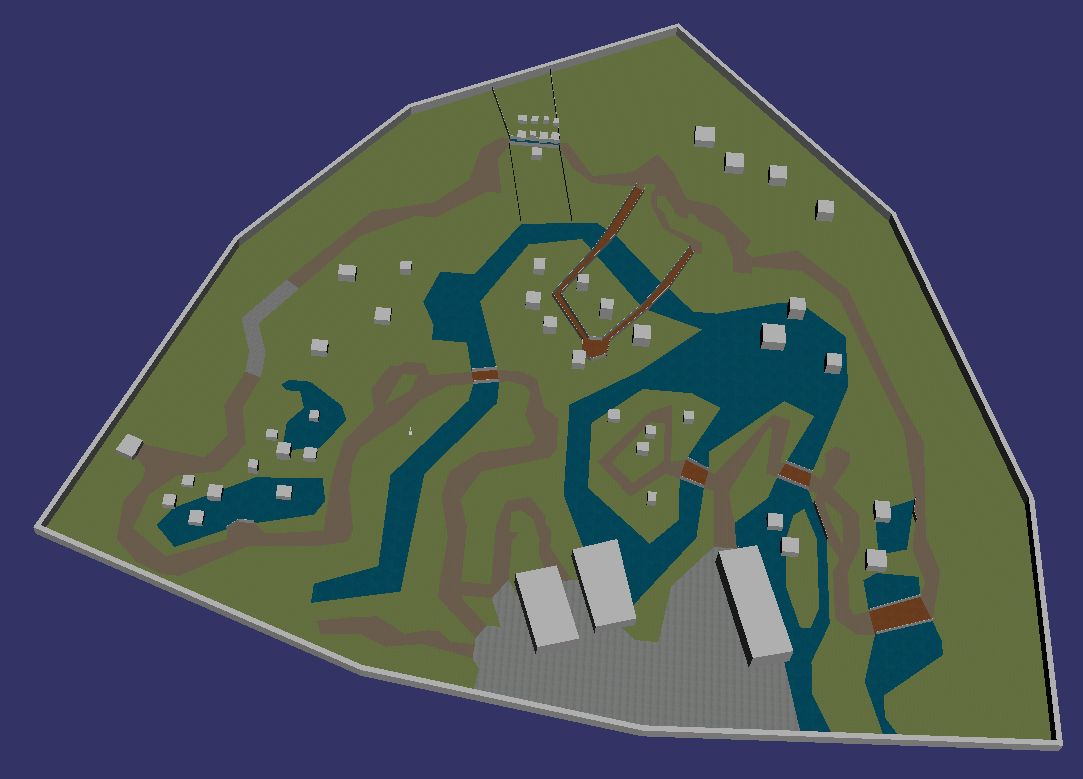
\includegraphics[width=\columnwidth]{images/zoo}
  \caption{The zoo is a remodelling of the Zoo Leipzig.}
\end{figure}

\column{0.5\textwidth}
\begin{figure}
	\centering
	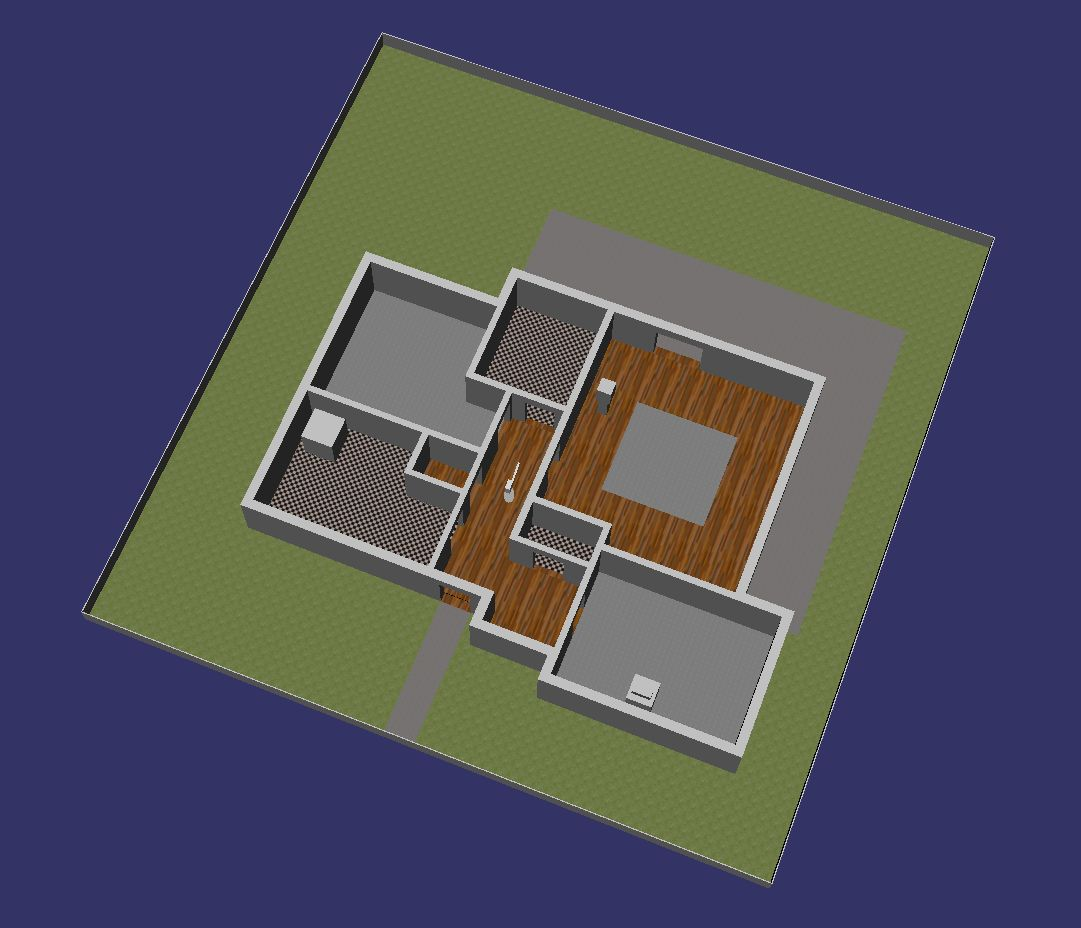
\includegraphics[width=\columnwidth]{images/apartment}
	\caption{Layout of a standard apartment in Halle.}
\end{figure}

\end{columns}

\end{frame}

\section{User Study}

\subsection{Study Design}

\begin{frame}{Study Design}

\alert{Participants:} 6 participants (5 male, 1 female) between 20
and 40 years
\begin{block}{Procedure}
\begin{enumerate}
  	\item Questions before the experiment
  	\item Familiarize with controls (with vision)
  	\item Solve different tasks (blindfolded)
  	\item Questions after the experiment 
  \end{enumerate}
\end{block}

\begin{block}{Questionnaire}
\begin{itemize}
  	\item Assess perceived difficulty of daily tasks
  	\item Assess perceived usefulness of different senses and cues 
  \end{itemize}
\end{block}

\end{frame}

\subsection{Results}

\begin{frame}{Results}

\begin{figure}[tb]
\centering

\begin{tikzpicture}

\tikzstyle{every node}+=[font=\sffamily,align=center,font=\small]

\begin{axis}[
width=0.8\textwidth, height=0.61\textwidth,
ymajorgrids=true, yminorgrids=true,
ybar,
xtick=data,
bar width=20pt,
enlarge x limits=0.15,
%xlabel={Task},
ylabel={Increase in rated difficulty\\ (5 level scale)}
]

\addplot[fill=black!20,draw=black!80,
error bars/.cd, y explicit, y dir=both] coordinates {
(1,0.5)+-(0,0.547722558)
(2,0.833333333)+-(0,0.752772653)
(3,-1)+-(0,1.414213562)
(4,0.5)+-(0,0.836660027)
};

\end{axis}

\end{tikzpicture}

\caption{(1) ``crossing a street'', (2) ``walking in a park'', (3) ``navigating in an unknown apartment'',
and (4) ``navigating in a known apartment''.}
\label{fig:results}
\end{figure}

\end{frame}

\section{Conclusions}

\begin{frame}{Conclusions}
Problems with the navigation:
\begin{itemize}
  \item With just audio: very difficult
  \item With audio and assistance: too easy
  \item[$\Rightarrow$] Need force-feedback to allow more freedom
\end{itemize}
\vspace{0.5em}
\pause
Future directions:
\begin{itemize}
  \item Use 6 DOF force-feedback device like the
  \textsc{PHANTOM}\footnote{\url{http://www.sensabledental.com/}}
  \item More intuitive and realistic use of the cane
  \item Create more realistic scenarios (more freedom)
  \item[$\Rightarrow$] Engaging experience comparable to \textsc{Dialogue in the
  Dark}.
\end{itemize}
\end{frame}

\usebackgroundtemplate{\parbox[b][
\paperheight+1.45cm
]{
\paperwidth+1.45cm
}{
\hfill\tikz 
\node {
\includegraphics[width=0.55\textwidth]{images/questions.png}} 
node[fill=white,path fading=south,fading angle=45]
{\phantom{
\includegraphics[width=0.55\textwidth]{images/questions.png}}}
node[fill=white,opacity=0.1]
{\phantom{
\includegraphics[width=0.55\textwidth]{images/questions.png}}}; }}

\begin{frame}

\begin{center}
\Large Thank you for your attention.\\[0.7em]
Do you have any questions?
\end{center}

\end{frame}

\end{document}
